\chapter{Pérdida de energía de iones en elementos pesados}

%%%%%%%%%%%%%%%%%%%%%%%%%%%%%%%%%%%%%%%%%%%%%%%%%%%%%%%%%%%%%%%%%%%%%%%%
\section{Introducción}
%%%%%%%%%%%%%%%%%%%%%%%%%%%%%%%%%%%%%%%%%%%%%%%%%%%%%%%%%%%%%%%%%%%%%%%%
\label{sec:intro}

El estudio de procesos de pérdida de energía por impacto de iones 
en sólidos es una poderosa herramienta en diversas áreas de la ciencia
básica y tecnología de materiales. Para energías de impacto superiores 
a unos pocos keV/amu, las partículas cargadas monoenergéticas que 
penetran algún material pierden su energía a través de una serie de 
colisiones inelásticas consecutivas, principalmente con blancos
electrónicos~\cite{Chu:01,Sigmund:06}. La información proporcionada por 
el proceso de pérdida de energía es esencial no solo para tener una 
mejor comprensión de la física detrás de las interacciones fundamentales, 
sino también porque juega un papel fundamental en muchos campos 
aplicados como la ciencia de materiales, la física nuclear, la 
implantación iónica y la radioterapia~\cite{Sigmund:06,Schardt:10}. 
Tablas y códigos resultantes de cálculos semiempíricos están disponibles 
para una gran combinación de iones y objetivos~\cite{iaea_codes,Paul:03}. 
Sin embargo, datos experimentales y predicciones teóricas 
\textit{ab initio} son de crucial importancia para comprobar la 
fiabilidad de los modelos semiempíricos y determinación ciertos 
parámetros clave~\cite{Diwan:15,Damache:04,Damache:02} para la pérdida 
de energía media de iones por trayecto unitario $S(E)$. Los datos 
experimentales disponibles son a menudo bastante escasos para materiales 
correspondientes a elementos de baja presencia en la corteza superior de 
la Tierra. Por otro lado, los cálculos de dispersión inelástica de 
blancos pesados usando métodos de primeros principios constituyen una 
tarea difícil ya que se hace necesario tener en cuenta efectos 
relativistas. Éstos efectos son importantes no solo para definir el 
estado de los electrones internos sino también para determinar las 
energías de ligadura de las capas externas.

En este capítulo, examinaremos la estructura atómica de átomos pesados
y el proceso de pérdida de energía de iones cuando inciden sobre ellos.
Los métodos de Hartree--Fock, y su versión relativista Dirac--Fock, 
son las aproximaciones más conocidas para el cálculo de funciones 
radiales y energías orbitales. Éstos se basan en el principio 
variacional y pueden producir resultados muy precisos. Sin embargo, el 
principio variacional presenta varios inconvenientes: el precio de la 
precisión del método se paga con funciones de onda radiales dependientes 
de los términos, las cuales no son ortogonales entre configuraciones. 
Estas características hacen que el uso de las funciones de onda sea 
engorroso en el cálculo las transiciones radiativas y de colisión. Más 
aún, dado que el principio variacional implica la minimización de la 
energía total, las energías de transición entre niveles cercanos se 
obtienen como diferencias muy pequeñas entre números grandes, y los 
resultados son muy susceptibles a errores numéricos. Esto es 
especialmente importante para los átomos de carga nuclear $Z$ grandes 
porque la energía total es muy grande. 

El aproximación teórica implementada aquí para describir los blancos 
pesados fue desarrollada por Klapisch y colaboradores 
\cite{Klapisch:77,Koenig:72,Klapisch:71,Klapisch:67}. Este método
está basado en la combinación de la teoría de perturbaciones de primer 
orden y la aproximación de campo central. La ecuación de Dirac 
correspondiente para cada sistema se resuelve y se obtienen las 
funciones de onda de orden cero. El Hamiltoniano resultante es luego
diagonalizado en las bases de estas funciones implementando el método de
interacción de configuraciones~(\acs{ci}). El término de Breit y las 
correcciones debido a los efectos electrodinámicos cuánticos (\acs{qed}) 
se incluyen a las energías a segundo orden. Las funciones de onda y 
energías relativistas son implementadas para el cálculo de pérdida de 
energía. 
%Diversos métodos consideran la descripción del estado inicial del blanco como datos de entrada para el cálculo de procesos inelásticos. Por ejemplo, la aproximación de plasma local por capa (\acs{slpa}) permite calcular los diferentes momentos de pérdida de energía~\cite{Montanari:13,Montanari:09,Montanari:11,Oswald:18} conociendo solo las densidades orbitales y las energías de enlace de los electrones objetivo en el estado fundamental.
La descripción de blancos pesados que cuentan con electrones en la capa 
$4f$ es particularmente importante ya que estos electrones tiene un rol 
fundamental en la predicción de pérdida de energía a energías 
bajas~\cite{Roth:17}. 

El enfoque teórico implementado en el cálculo de pérdida de energía 
utiliza la aproximación de plasma local por capa (\acs{slpa}) 
\cite{Montanari:13} para describir la energía transferida a los 
electrones ligados $1s$-$4f$ y dos modelos diferentes para el gas de 
electrones libre (\acs{feg}); en la región de baja energía, el modelo 
de potencial apantallado con condición de cúspide (\acs{spcc}) 
\cite{Montanari:17}, que está basado en un formalismo binario no lineal, 
y el formalismo dieléctrico de Mermin-Lindhard (\acs{dielectric-ml}) 
\cite{Mermin:70} para energías alrededor del frenado máximo y 
superiores. Este modelo requiere conocer las funciones de onda 
relativistas y energías de ligadura del blanco, considerando un cierto 
número de electrones de las capas externas en el FEG~\cite{Mendez:19}. 
% El hafnio es particularmente interesante ya que la subcapa 4f (con 14 electrones) es el principal contribuyente por debajo del FEG, lo que hace que las secciones eficaces de frenado sean muy sensibles a una buena descripción de esta capa. Se ha considerado el apantallamiento entre los electrones 4f y 5p y se ha descubierto que juega un papel importante en los cálculos de SLPA.

En este capítulo estudiaremos tres grupos de átomos de la tabla 
periódica: metales de transición con electrones de la capa $4d$ como 
valencia (Zr y Pd), lantánidos con la capa $4f$ abierta (Gd y Er), 
y metales de transición pesados con la capa $4f$ completa (Hf y Pt). 

{\color{red} Escribir sobre las aplicaciones de los blancos que voy a 
tratar: Zr, Pd, Hf, Pt, Gd y Er  (ver paper de Moro).}

%So far, only one experimental work has been published regarding the stopping power cross section of pure hafnium for protons~\cite{Sirotinin}, while more attention has been recently given to studies involving hafnium oxide due to its practical use~\cite{Abril,Behar,Primetzhofer,Roth}. It is well known that significant attention has been paid in recent years to transition metal-oxides such as HfO$_2$ because of their potential as alternative gate dielectrics to replace SiO$_2$ for the future generation of nano-electronics with less than 45 nm gate length~\cite{Choi,Robertson}. Some important physical properties of the above mentioned metal-oxide films depend on their thickness, which is often measured by using Rutherford Backscattering Spectrometry~\cite{Alfassi01,Tesmer01}. This method relies on the determination of both the scattering cross section and also the stopping power of ion beams in the material of interest.

%In this study, we report experimental stopping power cross sections over the incident energy range (0.6-2.5) MeV for protons crossing self-supported Hf thin-film by using the transmission method. We aim not only to upgrade stopping power data compilations~\cite{HPaul03,mondim17} but also to provide useful information about the processes governing the slowing down of protons in multi-electronic targets. In the rare earth metals, the $4f$ electrons play an essential role in the stopping power since they belong to the first shell of bound electrons below the conduction band. As already noted \cite{Roth17}, the free electron gas (FEG) shows unexpected behavior in these elements, which casts doubts on its proper description. In the case of Hf, we found the contribution of the $4f$-shell to be decisive even at impact energies around the stopping maximum, as will be shown later.

Los detalles teóricos del cálculo de los blancos relativistas a estudiar 
se dan en la sección~\ref{sec:blancos-relat}. Los modelos teóricos 
implementados para la predicción de la pérdida de energia se detallan 
en la sección~\ref{sec:slpa+feg}. Los resultados obtenidos teóricamente 
para los blancos Hf, Pt, Ta, y Gd, los cuales son comparados con valores 
experimentales. Además, comparamos nuestras predicciones con los 
modelos teóricos de Grande y Schiwietz~\cite{Grande:01,casp52}, y de 
Sigmund y Schinner~\cite{DPASS20}. Debido a su gran implementación en 
diversas aplicaciones, también consideramos los valores semi-empiricos 
dados por el paquete SRIM-2013~\cite{Ziegler01} y las tablas 
ICRU-49~\cite{ICRU49}. Las conclusiones se encuentran al final del capítulo,
en la sección~\ref{sec:stopping-conclusiones}.

%%%%%%%%%%%%%%%%%%%%%%%%%%%%%%%%%%%%%%%%%%%%%%%%%%%%%%%%%%%%%%%%%%%%%%%%
\section{Descripción de blancos relativistas}
%%%%%%%%%%%%%%%%%%%%%%%%%%%%%%%%%%%%%%%%%%%%%%%%%%%%%%%%%%%%%%%%%%%%%%%%
\label{sec:blancos-relat}

La descripción de los estados de átomos pesados relativistas se 
obtiene resolviendo el Hamiltoniano de Dirac multielectrónico
\begin{equation}
 H = H' + H_{\mathrm{\mbox{\scriptsize Breit}}}(i,j) +
 H_{\mbox{\scriptsize QED}}\,,
\label{eq:htot}
\end{equation}
donde $H_{\mathrm{\mbox{\scriptsize Breit}}}(i,j)$ es el término de 
Breit, $H_{\mbox{\scriptsize QED}}$ considera los efectos 
electrodinámicos cuánticos (\acs{qed}), y
\begin{equation}
 H' = \sum_i \left[ h_i^{\mbox{\scriptsize D}} - \frac{Z}{r_i}\right]
 + \sum_{i<j}\frac{1}{r_{ij}}\,,
\label{eq:hprim}
\end{equation}
siendo $h_i^{\mbox{\scriptsize D}}$ el término cinético del 
Hamiltoniano de Dirac de una partícula. Los términos restantes en la
ecuación~(\ref{eq:hprim}) corresponden a las interacciones 
núcleo--electrón y electrón--electrón, respectivamente. Usando la 
aproximación de campo central y mediante la introducción de un potencial 
paramétrico $U(\boldsymbol{\alpha},r)$, el Hamiltoniano $H'$ se puede escribir como la 
combinación de un término de orden cero, 
\begin{equation}
 H_0 = \sum_i h_i^{\mbox{\scriptsize D}} + U(\boldsymbol{\alpha},r_i)\,,
\end{equation}
más una pequeña perturbación
\begin{equation}
 H_1 = \sum_{i<j}\frac{1}{r_{ij}}
 - \sum_i \left[ \frac{Z}{r_i} + U(\boldsymbol{\alpha},r_i) \right]\,.
\end{equation}
Las soluciones de espinor de cuatro componentes de un electrón de la 
ecuación de Dirac
\begin{equation}
\left[ h_i^{\mbox{\scriptsize D}} +U(\boldsymbol{\alpha},r) \right] \varphi_{nljm}(\mathbf{r}) 
= \varepsilon_{nljm} \varphi_{nljm}(\mathbf{r})\,,
\label{eq:ecuacionDirac}
\end{equation}
llamadas orbitales relativistas, pueden ser caracterizadas por un 
conjunto de números cuánticos $nljm$, donde $l$ es el número cuántico 
del momento angular orbital de las componentes superiores. 
% componentes superiores = upper components ???

La solución de orden cero de un sistema $N$--electrónico se construye a 
partir de productos antisimetrizados de orbitales en cualquier esquema 
de acoplamiento elegido $\Gamma JM$ como 
\begin{equation}
\Psi_{\Gamma}\left(\mathbf{r}_1, \mathbf{r}_2, \ldots, \mathbf{r}_N\right)=A \sum_{all\,\,m}\left\langle\Gamma J M \mid m_1 m_2, \ldots, m_{N}\right\rangle \prod_{a} \varphi_{n_a l_a j_a m_a}\left(\mathbf{r}_a\right)\,,
\end{equation}
donde $A$ es el operador de antisimetría. Los estados y niveles 
específicos se denotan $\Gamma_iJ_iM_i$ y $\Gamma_iJ_i$, respectivamente,
donde $\Gamma_i$ representa el conjunto de números cuánticos necesario 
para identificar el estado de manera únivoca. 

Una configuración 
$C\equiv\prod_{a=1}^N\mathbf{j}_a=\prod_{i=1}\mathbf{j}_i^{q_i}$ es un 
conjunto de estados degenerados, con valores fijos $\mathbf{j}_i=n_il_ij_i$
y números de ocupación $q_i$, todos con energías de orden cero 
$E_C^0=\prod_{i=1}\,q_i\varepsilon_i$. 
El Hamiltoniano $H'$ se construye sobre la base de las configuraciones 
elegidas obtenidas con el potencial paramétrico. Luego, la matriz es 
diagonalizada, produciendo estados de configuración mixtos y energías 
de primer orden con algunas correcciones de correlación. Las funciones 
de onda resultantes se utilizan para agregar las correcciones QED y el 
término de Breit a las energías como perturbaciones de segundo orden.

La idea detrás del potencial paramétrico $U(\boldsymbol{\alpha},r)$ es 
describir de manera simple el apantallamiento de la distribución de carga 
de los electrones usando una expresión paramétrica analítica, donde 
$\boldsymbol{\alpha}=\left\{\alpha_1,\alpha_2,\ldots,\alpha_k\right\}$ 
es un conjunto de parámetros que se definen mediante la optimización 
del sistema y $k$ es el número de capas ocupadas. Aplicando la ecuación de 
Poisson a la densidad de carga radial de los $q$ electrones descritos 
por los orbitales de tipo Slater
\begin{equation}
\rho(r) = -4\pi r^2 qN\left|r^{l+1}e^{-\alpha r/2}\right|^2\,,
\end{equation} 
con las condiciones de borde 
\begin{equation}
U(\boldsymbol{\alpha},r\rightarrow\infty)=Z-\frac{q}{r}\,.
\end{equation} 
Aquí, $N$ es un factor de normalización, y $\alpha_i$ está relacionado 
con el radio medio de la capa tal que $\alpha_i=(2l+3)/\langle r\rangle_i$. 
Es necesario mostrar que el potencial para diversas capas y el nucleo 
se puede escribir como
\begin{equation}
U(\boldsymbol{\alpha},r)=-\frac{1}{r} \left[I+\sum_s q_s\, g(L_s,\alpha_s,r) 
+ \sum_t q_t\,f(l_t,\alpha_t,r)\right]\,,
\label{eq:potparam}
\end{equation}
donde los índices $s$ y $t$ recorren las capas cerradas y abiertas, 
respectivamente. El valor $I$ es el grado de ionización más uno. 
%Esto elimina la auto-interacción adicional de los electrones ligados. Aquí, $\boldsymbol{\alpha}$ representa un conjunto de parámetros $\left\{\alpha_s,\alpha_t\right\}$ que describen el radio medio de las capas. 
Las funciones $f$ y $g$ son tales que
\begin{eqnarray}
f(l,\alpha,r)&=&\mathrm{e}^{-\alpha r} \sum_{j=1}^{2 l+1}\left(1-\frac{j}{2 l+2}\right) \frac{(\alpha r)^{j}}{j !}\,, \\
g(L, \alpha, r)&=&\frac{1}{2 n^{2}} \sum_{l=0}^{L=n-1}(4 l+2) f\left(l, \alpha^{(l)}, r\right)\,,
\end{eqnarray}
donde $n$ es el número cuántico principal y $\alpha^{(l)}$ incluye una
corrección para la ligera diferencia en el radio debido al número del
momento angular cuántico de las subcapas. 
Los parámetros libres $q$ son el número efectivo de electrones en la 
capa y satisfacen $I+\sum_{s} q_{s}+\sum_{t} q_{t}=Z$. 

Esta parametrización resulta en que cualquier cantidad atómica calculada 
con las funciones de onda dadas por la ecuación~(\ref{eq:ecuacionDirac}) 
junto con el potencial~(\ref{eq:potparam}) se convierte en una función 
numérica de los parámetros. Hay múltiples formas posibles de elegir los 
parámetros $\boldsymbol{\alpha}$, de acuerdo a diversos criterios 
teóricamente válidos. Entre ellos, podemos nombrar tres;
\begin{itemize}
\item criterio espectroscópico: minimización de la desviación \acs{rms} 
entre los niveles de energía teóricos y experimentales,
\item criterio variacional: minimización de la energía total, y
\item criterio perturbacional: minimización del Hamiltoniano perturbativo
$H_1$. % primer orden de las energías de configuración promedio (\acs{ca}), 
\end{itemize}
%Uno de ellos es la minimización de primer orden de las energías de configuración promedio (\acs{ca}), o de las energías de cualquier conjunto de niveles elegido. Otra posibilidad es minimizar la desviación \acs{rms} entre los niveles de energía teóricos y experimentales. 
En nuestro trabajo implementamos la optimización perturbativa de primer 
orden, donde se implementa la minimización de las energías de 
configuración promedio (\acs{ca}), o de las energías de cualquier 
conjunto de niveles elegido. Dado que las energías de primer orden 
sobre las que actúa la optimización incluyen la contribución de 
intercambio exacta, los parámetros resultantes absorben el efecto del 
intercambio y, por lo tanto, no hay necesidad de un potencial de 
intercambio adicional explícito.

Por otro lado, siendo $U(\boldsymbol{\alpha},r)$ un potencial central,
es posible plantear la separación de variables esféricas de las 
soluciones de la ecuación de Dirac~(\ref{eq:ecuacionDirac}), tal que
\begin{equation}
\varphi_{nljm}(\mathbf{r}) = \frac{1}{r} \left( 
\begin{array}{c}
i P_{nlj}(r) \,\Omega_{jlm}(\hat{\mathbf{r}}) \\ 
  Q_{nlj}(r) \,(\boldsymbol{\sigma}\cdot\hat{\mathbf{r}})\,\Omega_{jlm}(\hat{\mathbf{r}})
\end{array}
\right)\,,
\label{eq:sepespinor}
\end{equation}
donde $P_{nlj}(r)$ y $Q_{nlj}(r)$ son los componentes fuerte y débil de los 
espinores de Dirac, respectivamente. Los espinores esféricos 
$\Omega_{jlm}(\hat{\mathbf{r}})$ son autoestados de $J^2$ y $J_z$ a 
través de la relación
\begin{equation}
\Omega_{j, l, m}(\theta, \phi)=\sum_{\mu} C(l, 1 / 2, j ; m-\mu, \mu, m) Y_{l, m-\mu}(\theta, \phi) \chi_{\mu}\,,
\end{equation}
donde $C\left(j_{1}, j_{2}, j ; m_{1}, m_{2}, m\right)$ son los
coeficientes de Clebsch--Gordan. Así, el valor esperado de cualquier 
operador $\hat{A}$ estará dado por
\begin{equation}
\langle\hat{A}\rangle=\int_0^{\infty}\left[P^*(r)\,\hat{A}\,P(r) 
 +Q^*(r)\,\hat{A}\,Q(r)
\right]\,dr\,.
\label{eq:meanvalr}
\end{equation}
Para los orbitales relativistas, usamos la notación $nl\pm$, que 
significa $nlj$, donde el índice $j=l\pm1/2$ se representa como $\pm$.

%%%%%%%%%%%%%%%%%%%%%%%%%%%%%%%%%%%%%%%%%%%%%%%%%%%%%%%%%%%%%%%%%%%%%%%%
\subsection{Energía de ligadura y valores medios}
%%%%%%%%%%%%%%%%%%%%%%%%%%%%%%%%%%%%%%%%%%%%%%%%%%%%%%%%%%%%%%%%%%%%%%%%

Los efectos de la interacción de configuraciones (\acs{ci}) son muy 
importantes en el caso de los átomos relativistas. Así, la correcta 
descripción del blanco depende de las configuraciones consideradas en 
el CI. En esta sección, la optimización de los blancos consiste en la 
determinación de las configuraciones que contribuyen de manera 
significativa a la mezcla en la interacción de configuraciones. 
La ecuación de Dirac dada por la ecuación~(\ref{eq:ecuacionDirac}) fue 
resuelta numéricamente usando el paquete de códigos 
{\sc hullac}~\cite{BarShalom:01}. En este conjunto de programas 
computacionales, el código {\sc relac} permite calcular las energías 
relativistas y funciones de onda orbitales en primer orden usando el 
método potencial paramétrico descrito en la sección anterior. 

\begin{table*}[t]
\centering
\begin{tabular}{|c|c|c|c|l|}
\hline
Grupo & Nombre   & Símbolo & $Z$ & Config. fundamental \\
\hline
\hline
\multirow{2}{*}{A} & Circonio & Zr & 40 & [Kr]~$4d^2\,5s^2$ \\
                   & Paladio  & Pd & 46 & [Kr]~$4d^{10}$ \\
\hline
\multirow{2}{*}{B} & Gadolinio & Gd & 64 & [Xe]~$4f^7\,5d\,6s^2$ \\
                   & Erbio     & Er & 68 & [Xe]~$4f^{12}\,6s^2$ \\
\hline
\multirow{2}{*}{C} & Hafnio  & Hf & 72 & [Xe]~$4f^{14}\,5d^2\,6s^2$ \\
                   & Platino & Pt & 78 & [Xe]~$4f^{14}\,5d^9\,6s$ \\
\hline
\end{tabular}
\caption[Blancos relativistas y sus configuraciones fundamentales]
{Blancos relativistas y sus configuraciones fundamentales.}
\label{tab:gruposrelat} 
\end{table*}

Los elementos que examinamos en esta sección son divididos en tres 
grupos según el período de la tabla periódica al que pertenecen. La 
clasificación de estos blancos y sus configuraciones fundamentales se
muestran en la tabla~\ref{tab:gruposrelat}. El grupo A está compuesto 
por los metales de transición Zr y Pd, mientras que Hf y Pt pertenecen 
al grupo C. Los lantánidos Gd y Er conforman el grupo B. 
Podemos escribir una fórmula general para la configuración fundamental 
de los metales de transición, 
\begin{equation}
nd^w\,(n+1)s^x\,,
\end{equation}
donde $n=4$, $w=2,10$, $x=2,0$ para el grupo A, y $n=5$, $w=2,9$, 
$x=2,1$ para el grupo B. Los electrones $nd$ y $(n+1)s$ tienen energías 
de ligadura similares. Por lo tanto, las configuraciones 
\begin{gather}
nd^w(n+1)s^2, \\
nd^{w+1}(n+1)s, \\
nd^{w+2}
\end{gather}
tienen energías comparables. Dado que estas configuraciones tienen la 
misma paridad, éstas cumplen los dos requerimientos mencionados 
anteriormente, y son fundamentales en los cálculos de mezcla de 
configuraciones. Entonces, por ejemplo, en el cálculo de la estructura 
de Zr, además del estado fundamental del átomo [Kr]~$4d^2\,5s^2$ 
incluimos en la mezcla las configuraciones $4d^2\,5s^2$, $4d^3\,5s$, y 
$4d^4$. De manera similar, para el átomo de Pt, las configuraciones
[Xe]~$5d^9\,6s$ y $5d^{10}$ son consideradas en el cálculo relativista.

La configuración fundamental de los lantánidos del grupo C tiene la 
forma 
\begin{equation}
nf^w\,(n+1)d^x\,(n+2)s^y\,,
\end{equation}
donde $n=4$, $w=7,12$, $x=1,0$ y $y=2,2$. En el caso de Gd, también 
tenemos que incluir las interacciones entre los electrones de las capas
$4f$ y $5d$, que están abiertas. Así, las contribuciones más 
importantes a la interacción de configuraciones están dadas por la 
mezcla de las configuraciones $4f^7\,5d\,6s^2$ y $4f^8\,6s^2$.
Para Er, la mayor mezcla es producida por las configuraciones 
$4f^{12}\,6s^2$ y $4f^{12}\,5d\,6s$.

Los valores teóricos optimizados de energías de ligadura para los 
blancos relativistas de la tabla~\ref{tab:gruposrelat} se dan en la 
tabla~\ref{tab:relatresults} y se muestran en la 
figura~\ref{fig:bindener} con diamantes rellenos. 
En la tabla se incluyen los valores medios $\langle r\rangle$ de cada 
capa, los cuales se obtienen a partir de la ecuación~(\ref{eq:meanvalr}). 
Datos experimentales de los blancos en estado sólido~\cite{Williams:95}
se presentan usando círculos vacíos. Los resultados obtenidos por 
Desclaux~\cite{Desclaux:73} mediante la implementación del método 
de Dirac--Fock se muestran en la figura con símbolos $\times$.

\begin{figure}[t]
\centering
\includegraphics[width=\textwidth]{heavy/bindener.eps}
\caption[Energías de ligadura de blancos relativistas]
{Energías de ligadura de Zr, Pd, Gd, Er, Hf y Pt. Símbolos: 
$\blacklozenge$ resultados teóricos del presente trabajo, 
$\times$ valores teóricos del método Dirac--Fock~\cite{Desclaux:73}, y 
$\medcircle$ datos experimentales en sólidos~\cite{Williams:95}.}
\label{fig:bindener}
\end{figure}


\begin{tabularx}{\textwidth}{|c|YYY|YYY|YYY|}
\caption[Energías de ligadura y valores $\langle r \rangle$ de blancos
relativistas]
{Energías de ligadura teóricas y experimentales~\cite{Williams:95} de 
Zr, Pd, Gd, Er, Hf y Pt. Valores medios $\langle r \rangle$ en a.u. 
obtenidos a partir de la ecuación~(\ref{eq:meanvalr}).}
\label{tab:relatresults} \\
\hline
%% primer encabezado
\multirow{2}{*}{$nlj$} 
 & $E^{\mbox{\tiny exp}}$
 & $E^{\mbox{\tiny teo}}$
 & $\langle r\rangle^{\mbox{\tiny teo}}$ 
 & $E^{\mbox{\tiny exp}}$
 & $E^{\mbox{\tiny teo}}$
 & $\langle r\rangle^{\mbox{\tiny teo}}$
 & $E^{\mbox{\tiny exp}}$
 & $E^{\mbox{\tiny teo}}$
 & $\langle r\rangle^{\mbox{\tiny teo}}$  \\
\endfirsthead % fin de primer encabezado
%% segundo encabezado (tabla continuada)
\caption*{Tabla x.2 (Cont.): 
Energías de ligadura teóricas y experimentales~\cite{Williams:95} de 
Zr, Pd, Gd, Er, Hf y Pt. Valores medios $\langle r \rangle$ en a.u. 
obtenidos a partir de la ecuación~(\ref{eq:meanvalr}).} \\
\hline
$nlj$ 
 & $E^{\mbox{\tiny exp}}$
 & $E^{\mbox{\tiny teo}}$
 & $\langle r\rangle^{\mbox{\tiny teo}}$ 
 & $E^{\mbox{\tiny exp}}$
 & $E^{\mbox{\tiny teo}}$
 & $\langle r\rangle^{\mbox{\tiny teo}}$
 & $E^{\mbox{\tiny exp}}$
 & $E^{\mbox{\tiny teo}}$
 & $\langle r\rangle^{\mbox{\tiny teo}}$  \\
\hline
\endhead % fin de segundo encabezado
\hline
\endfoot % lineas que cierran la tabla 
  \cline{2-10}
  & \multicolumn{3}{c}{Zr} &  \multicolumn{3}{c}{Gd} & \multicolumn{3}{c}{Hf} \\
\hline
$1s$   & 661.45 & 651.34 & 0.0372 & 1846.2 & 1843.6 & 0.0219 & 2401.6 & 2400.4 & 0.0190 \\
$2s$   & 93.05  & 90.40  & 0.163  & 307.8  & 303.0  & 0.0929 & 414.20 & 408.98 & 0.0798 \\
$2p_-$ & 84.79  & 82.78  & 0.139  & 291.4  & 287.2  & 0.0776 & 394.65 & 390.26 & 0.0662 \\
$2p_+$ & 81.70  & 79.66  & 0.144  & 266.2  & 261.6  & 0.0845 & 351.4  & 346.4  & 0.0740 \\
$3s$   & 15.82  & 14.76  & 0.460  & 69.13  & 67.43  & 0.244  & 95.58  & 93.55  & 0.208 \\
$3p_-$ & 12.62  & 11.95  & 0.456  & 62.03  & 60.79  & 0.234  & 86.91  & 85.40  & 0.198 \\
$3p_+$ & 12.12  & 11.45  & 0.467  & 56.74  & 55.50  & 0.247  & 77.43  & 75.97  & 0.213 \\
$3d_-$ & 6.656  & 6.505  & 0.450  & 44.904 & 44.084 & 0.219  & 63.06  & 62.14  & 0.187 \\
$3d_+$ & 6.571  & 6.413  & 0.454  & 43.717 & 42.953 & 0.223  & 61.08  & 60.12  & 0.191 \\
$4s$   & 1.86   & 1.99   & 1.20   & 13.91  & 13.50  & 0.553  & 19.8   & 18.8   & 0.468 \\
$4p_-$ & 1.05   & 1.21   & 1.32   & 10.5   & 10.9   & 0.565  & 16.10  & 15.45  & 0.474 \\
$4p_+$ & 0.996  & 1.14   & 1.36   & 9.96   & 9.74   & 0.596  & 13.99  & 13.28  & 0.508 \\
$4d_-$ &        & 0.103  & 3.15   & -      & 5.515  & 0.634  & 8.08   & 7.81   & 0.530 \\
$4d_+$ &        & 0.100  & 3.29   & 5.240  & 5.306  & 0.645  & 7.772  & 7.418  & 0.542 \\
$5s$   &        & 0.182  & 4.34   & 1.3    & 2.0    & 1.34   & 2.36   & 2.55   & 1.12 \\
$5p_-$ &        &        &        & 0.74   & 1.3    & 1.51   & 1.4    & 1.6    & 1.24 \\
$5p_+$ &        &        &        & 0.74   & 1.2    & 1.60   & 1.10   & 1.28   & 1.35 \\
$4f_-$ &        &        &        & 0.32   & 0.41   & 0.916  & 0.584  & 0.725  & 0.666 \\
$4f_+$ &        &        &        & 0.32   & 0.38   & 0.934  & 0.522  & 0.660  & 0.679 \\
$6s$   &        &        &        &        & 0.31   & 3.70   &        & 0.214 & 3.83 \\
$5d_-$ &        &        &        &        & 0.29   & 2.50   &        & 0.125 & 2.77 \\
$5d_+$ &        &        &        &        & 0.28   & 2.56   &        & 0.109 & 3.13 \\
\hline
  & \multicolumn{3}{c}{Pd} &  \multicolumn{3}{c}{Er} & \multicolumn{3}{c}{Pt} \\
\hline
$1s$   & 894.84 & 880.77 & 0.0320 & 2112.7 & 2114.2 & 0.0203 & 2880.9 & 2881.6 & 0.0171 \\
$2s$   & 132.44 & 128.73 & 0.138  & 358.4  & 353.7  & 0.0858 & 510.08 & 504.78 & 0.0718 \\
$2p_-$ & 122.37 & 119.68 & 0.117  & 340.5  & 337.5  & 0.0712 & 487.77 & 483.25 & 0.0591 \\
$2p_+$ & 116.60 & 113.89 & 0.122  & 307.2  & 303.3  & 0.0785 & 424.97 & 419.70 & 0.0676 \\
$3s$   & 24.68  & 23.16  & 0.382  & 81.07  & 79.34  & 0.225  & 121.1  & 118.8  & 0.187 \\
$3p_-$ & 20.58  & 19.52  & 0.374  & 73.72  & 72.00  & 0.215  & 111.2  & 109.4  & 0.177 \\
$3p_+$ & 19.56  & 18.53  & 0.385  & 66.59  & 64.92  & 0.229  & 97.20  & 95.37  & 0.192 \\
$3d_-$ & 12.51  & 11.98  & 0.359  & 53.40  & 51.91  & 0.202  & 80.92  & 79.83  & 0.168 \\
$3d_+$ & 12.32  & 11.78  & 0.363  & 51.78  & 50.38  & 0.207  & 77.98  & 76.83  & 0.172 \\
$4s$   & 3.20   & 3.23   & 0.937  & 16.53  & 15.62  & 0.507  & 26.66  & 25.53  & 0.416 \\
$4p_-$ & 2.05   & 2.09   & 1.01   & 13.46  & 12.69  & 0.515  & 22.38  & 21.55  & 0.419 \\
$4p_+$ & 1.87   & 1.92   & 1.04   & 11.77  & 11.06  & 0.548  & 19.09  & 18.22  & 0.453 \\
$4d_-$ &        & 0.216  & 1.61   & 6.160  & 6.186  & 0.578  & 12.19  & 11.70  & 0.463 \\
$4d_+$ &        & 0.198  & 1.67   & 6.160  & 5.892  & 0.589  & 11.56  & 11.09  & 0.474 \\
$5s$   &        &        &        & 1.86   & 1.95   & 1.25   & 3.737  & 3.829  & 0.942 \\
$5p_-$ &        &        &        & 1.15   & 1.16   & 1.41   & 2.40   & 2.53   & 1.02 \\
$5p_+$ &        &        &        & 0.908  & 0.954  & 1.52   & 1.90   & 1.94   & 1.12 \\
$4f_-$ &        &        &        & -      & 0.18   & 0.813  & 2.74   & 2.75   & 0.513 \\
$4f_+$ &        &        &        & 0.17   & 0.14   & 0.838  & 2.62   & 2.62   & 0.520 \\
$6s$   &        &        &        &        & 0.19   & 4.33   &        & 0.250  & 3.30 \\
$5d_-$ &        &        &        &        & 0.080  & 4.91   &        & 0.250  & 1.71 \\
$5d_+$ &        &        &        &        & 0.076  & 5.45   &        & 0.200  & 1.88 \\
\end{tabularx}

En general, el acuerdo entre los presentes resultados teóricos y la
data experimental es muy bueno. Dado que la figura~\ref{fig:bindener} 
muestra las energías de enlace en un rango de magnitud de cinco órdenes, 
no es posible discernir las discrepancias entre los datos enumerados 
en la tabla~\ref{tab:relatresults} y los resultados del método de 
Dirac--Fock~\cite{Desclaux:73}. Para evaluar estas diferencias, las 
relaciones $E^{\mbox{\scriptsize exp}}/E^{\mbox{\scriptsize teo}}$ y 
$E^{\mbox{\scriptsize exp}}/E^{\mbox{\scriptsize \cite{Desclaux:73}}}$
entre las energías de ligadura experimentales y los dos métodos 
teóricos considerados se muestran en la figura~\ref{fig:ratios} con los 
mismos símbolos y líneas que en la figura~\ref{fig:bindener}. Las 
energías de enlace que obtuvimos para Zr muestran un acuerdo general de 
aproximadamente 4\% para todas las capas, excepto para la subvalencia 
$4p$. Asimismo, los resultados obtenidos para Hf coinciden con los 
valores experimentales en $\sim$~3\%, excepto en las subcapas $5p$ y 
$4f$. Los lantánidos Gd y Er también presentan concordancia de alrededor 
del 3\%, con excepción de las subcapas más externas $5s$, $5p$ y $4f$. 
Sorprendentemente, para los metales de transición Pd y Pt, cuyas 
subcapas $nd$ están más llenas, la concordancia es mejor que el 3\% 
para todas las subcapas, incluso la subvalencia $4p$ de Pd y la $5p$, 
$4f$ de Pt. En todos los casos, los presentes resultados describen los 
datos experimentales con mayor precisión que~\cite{Desclaux:73}.


\begin{figure}[t]
\centering
 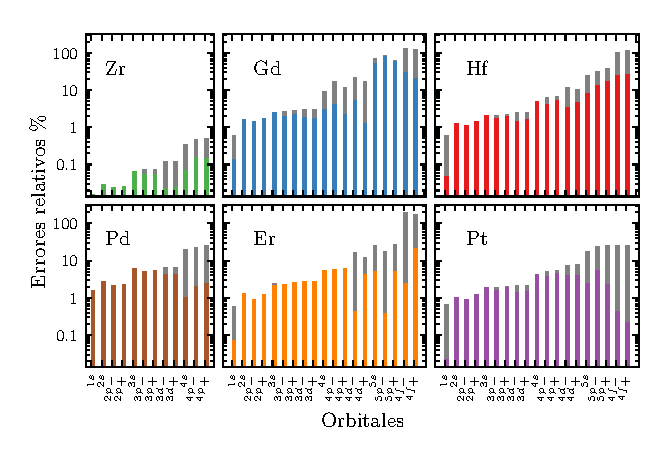
\includegraphics[width=\textwidth]{heavy/erp_heavy.eps} 
% 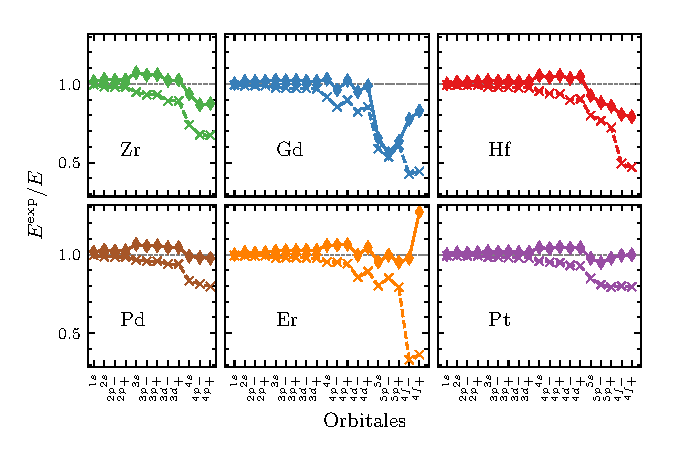
\includegraphics[width=\textwidth]{heavy/ratios_heavy.eps} 
\caption{Razón entre energías de ligadura experimentales and teóricas.}
\label{fig:ratios}
\end{figure}


\begin{comment}

\begin{tabularx}{\textwidth}{|c|YYY|YYY|YYY@{}|}
\caption[Energías de ligadura y valores $\langle r \rangle$ de blancos
relativistas]
{Energías de ligadura teóricas y experimentales~\cite{Williams:95} de 
Zr, Pd, Gd, Er, Hf y Pt. Valores medios $\langle r \rangle$ en a.u. 
obtenidos a partir de la ecuación~(\ref{eq:meanvalr}).}
\label{tab:relatresults} \\
\hline
%% primer encabezado
\multirow{2}{*}{$nljm$} 
 & $E^{\mbox{\tiny exp}}$
 & $E^{\mbox{\tiny teo}}$
 & $\langle r\rangle^{\mbox{\tiny teo}}$ 
 & $E^{\mbox{\tiny exp}}$
 & $E^{\mbox{\tiny teo}}$
 & $\langle r\rangle^{\mbox{\tiny teo}}$ \\
\endfirsthead % fin de primer encabezado
%% segundo encabezado (tabla continuada)
\caption*{Tabla x.2 (Cont.): 
Energías de ligadura teóricas y experimentales~\cite{Williams:95} de 
Zr, Pd, Gd, Er, Hf y Pt. Valores medios $\langle r \rangle$ en a.u. 
obtenidos a partir de la ecuación~(\ref{eq:meanvalr}).} \\
\hline
$nljm$ 
 & $E^{\mbox{\tiny exp}}$
 & $E^{\mbox{\tiny teo}}$
 & $\langle r\rangle^{\mbox{\tiny teo}}$ 
 & $E^{\mbox{\tiny exp}}$
 & $E^{\mbox{\tiny teo}}$
 & $\langle r\rangle^{\mbox{\tiny teo}}$ \\
\hline
\endhead % fin de segundo encabezado
\hline
\endfoot
\hline
\endfoot % lineas que cierran la tabla 
\cline{2-7}
       & \multicolumn{3}{c}{Zr} & \multicolumn{3}{c}{Pd} \\
\hline
$1s$   & 661.40 & 651.34 & 0.0372 & 894.83 & 880.77 & 0.032 \\
$2s$   & 93.05  & 90.40  & 0.163  & 132.4  & 128.7  & 0.138 \\
$2p^-$ & 84.78  & 82.78  & 0.139  & 122.4  & 119.7  & 0.117 \\
$2p^+$ & 81.69  & 79.66  & 0.144  & 116.6  & 113.9  & 0.122 \\
$3s$   & 15.81  & 14.76  & 0.460  & 24.68  & 23.16  & 0.382 \\
$3p^-$ & 12.62  & 11.95  & 0.456  & 20.58  & 19.52  & 0.374 \\
$3p^+$ & 12.12  & 11.45  & 0.467  & 19.56  & 18.53  & 0.385 \\
$3d^-$ & 6.656  & 6.505  & 0.450  & 12.51  & 11.98  & 0.359 \\
$3d^+$ & 6.571  & 6.413  & 0.454  & 12.32  & 11.78  & 0.363 \\
$4s$   & 1.86   & 1.99   & 1.20   & 3.20   & 3.23   & 0.937 \\
$4p^-$ & 1.05   & 1.21   & 1.32   & 2.05   & 2.09   & 1.01  \\
$4p^+$ & 0.996  & 1.14   & 1.36   & 1.87   & 1.91   & 1.04  \\
$4d^-$ &        & 0.103  & 3.15   &        & 0.216  & 1.61  \\
$4d^+$ &        & 0.100  & 3.29   &        & 0.198  & 1.67  \\
$5s$   &        & 0.182  & 4.34   &        &        &       \\
\hline
       &  \multicolumn{3}{c}{Gd} & \multicolumn{3}{c}{Er} \\
\hline
$1s$   & 1846.2 & 1834.6 & 0.0220 & 2112.5 & 2114.2 & 0.0203 \\
$2s$   & 307.8  & 303.1  & 0.0927 & 358.3  & 353.7  & 0.0859 \\
$2p^-$ & 291.4  & 288.9  & 0.0773 & 340.4  & 337.5  & 0.0714 \\
$2p^+$ & 266.2  & 263.2  & 0.0841 & 307.1  & 303.3  & 0.0788 \\
$3s$   & 69.12  & 67.00  & 0.245  & 81.07  & 79.34  & 0.225  \\
$3p^-$ & 62.03  & 60.48  & 0.234  & 73.72  & 72.00  & 0.215  \\
$3p^+$ & 56.74  & 55.29  & 0.247  & 66.59  & 64.92  & 0.229  \\
$3d^-$ & 44.903 & 43.633 & 0.219  & 53.40  & 51.91  & 0.202  \\
$3d^+$ & 43.716 & 42.492 & 0.224  & 51.78  & 50.38  & 0.206  \\
$4s$   & 13.91  & 13.36  & 0.554  & 16.53  & 15.62  & 0.507  \\
$4p^-$ & 10.5   & 10.8   & 0.565  & 13.46  & 12.69  & 0.516  \\ 
$4p^+$ & 9.96   & 9.65   & 0.596  & 11.77  & 11.06  & 0.549 \\
$4d^-$ & -      & 5.405  & 0.635  & 6.159  & 6.186  & 0.580 \\ 
$4d^+$ & 5.240  & 5.193  & 0.646  & 6.159  & 5.892  & 0.592 \\ 
$5s$   & 1.3    & 2.0    & 1.37   & 1.86   & 1.95   & 1.26   \\
$5p^-$ & 0.74   & 1.3    & 1.54   & 1.13   & 1.16   & 1.41  \\ 
$5p^+$ & 0.74   & 1.1    & 1.65   & 0.908  & 0.954  & 1.51  \\ 
$4f^-$ & 0.32   & 0.32   & 1.01   & -      & 0.18   & 0.851 \\ 
$4f^+$ & 0.32   & 0.30   & 1.05   & 0.17   & 0.14   & 0.876 \\ 
$6s$   &        & 0.40   & 3.79   &        & 0.19   & 3.43   \\
$5d^-$ &        & 0.35   & 2.77   &        &        &       \\ 
$5d^+$ &        & 0.34   & 2.84   &        &        &       \\ 
\hline
       & \multicolumn{3}{c}{Hf} & \multicolumn{3}{c}{Pt} \\
\hline
$1s$   & 2401.6 & 2400.4 & 0.0190 & 2880.9 & 2881.6 & 0.0171 \\
$2s$   & 414.19 & 408.98 & 0.0798 & 510.07 & 504.78 & 0.0718 \\
$2p^-$ & 394.64 & 390.26 & 0.0662 & 487.76 & 483.25 & 0.0591 \\
$2p^+$ & 351.4  & 346.4  & 0.0740 & 424.96 & 419.70 & 0.0676 \\
$3s$   & 95.58  & 93.55  & 0.208  & 121.1  & 118.8  & 0.187	\\
$3p^-$ & 86.91  & 85.40  & 0.198  & 111.2  & 109.4  & 0.177	\\
$3p^+$ & 77.43  & 75.97  & 0.213  & 97.20  & 95.37  & 0.192	\\
$3d^-$ & 63.06  & 62.14  & 0.187  & 80.92  & 79.83  & 0.168	\\
$3d^+$ & 61.08  & 60.12  & 0.191  & 77.98  & 76.83  & 0.172	\\
$4s$   & 19.8   & 18.8   & 0.468  & 26.66  & 25.53  & 0.416	\\
$4p^-$ & 16.10  & 15.46  & 0.474  & 22.38  & 21.55  & 0.419	\\
$4p^+$ & 13.99  & 13.28  & 0.508  & 19.09  & 18.22  & 0.453	\\
$4d^-$ & 8.08   & 7.81   & 0.530  & 12.19  & 11.70  & 0.463	\\
$4d^+$ & 7.772  & 7.418  & 0.542  & 11.56  & 11.09  & 0.474	\\
$5s$   & 2.36   & 2.55   & 1.12   & 3.737  & 3.829  & 0.942	\\
$5p^-$ & 1.4    & 1.6    & 1.24   & 2.40   & 2.53   & 1.02	\\
$5p^+$ & 1.10   & 1.28   & 1.35   & 1.90   & 1.94   & 1.12	\\
$4f^-$ & 0.584  & 0.725  & 0.666  & 2.74   & 2.75   & 0.513	\\
$4f^+$ & 0.522  & 0.660  & 0.679  & 2.62   & 2.62   & 0.520	\\
$6s$   &        & 0.214  & 3.83   &        & 0.250  & 3.30	\\
$5d^-$ &        & 0.125  & 2.27   &        & 0.250  & 1.71	\\
$5d^+$ &        & 0.109  & 3.13   &        & 0.200  & 1.88	\\
\end{tabularx}


\subsection{Discusión sobre valores para sólidos}

In this work, we calculated binding energies for isolated atoms (gases). 
However, the experimental energies considered for comparisons \cite{expdata}
correspond to measurements in solids (ionization of the bound electrons). 
As expected, the main gas--solid discrepancies are found for the outer 
shells. The electrons in the orbits adjacent to the conduction band
in a solid are loosely bound, compared to the tightly bounding
of the electrons in an isolated atom. The vertical dashed lines in Figs.~\ref{fig:fig1} and 
\ref{fig:fig2} separate the bound and the valence electrons.
The present results give a good insight about the number of electrons 
in the free electron gas (FEG) of solids, which 
are particularly relevant in stopping power calculations. 


The FEG is characterized by the density of electrons, or equivalently 
by the Wigner--Seitz radio $r_S$, directly related to the Fermi energy
$E_F$.
To obtain these values, a thorough analysis of the binding energies is
needed to determine the actual number of electrons belonging to the 
FEG. Our theoretical results for each target are displayed in 
Table~\ref{tab:tab3}.
For Zr, Nb, Hf, and Ta, the experimental $r_S$ are derived 
from the optical energy loss function \cite{werner,lynch,isaacson,romaniello},
resulting in $r_S^{\mbox{\scriptsize exp}}=2.18$, $1.72$, $2.12$ and $1.73$,
respectively. Our theoretical results agree within $4\%$ with these
values.
On the other hand, no experimental data was found for Gd and Er,
while for Pd, Os and Pt the number of electrons in the FEG are subject
of discussion. For example, for Pd, assuming that only 6 electrons belong
to the valence band (part of the $4d$ electrons), the Fermi energy is
$E_F=0.74$~a.u.. On the other hand, considering the whole subshell as
10 electrons in the conduction band, the corresponding
value is $E_F=1.02$~a.u. (displayed in Table~\ref{tab:tab3}).
Analogously, for Pt, assuming 6 valence
electrons (part of the $5d$ electrons) produces $E_F=0.72$~a.u., instead
of $E_F=1.02$~a.u., obtained with the assumption of 10 electrons 
belonging to the valence shell.


For the atoms studied here, we noted that the binding energies of the 
outermost electrons lay below the Fermi energies. However, the lower 
curves in Fig.~\ref{fig:fig2} show a clear contrast between the 
lanthanides and the rest of the atoms. 
For Gd, Table~\ref{tab:tab3} shows that the $4f$ electrons have very 
close energies to the outer $5d$ and $6s$ subshells. This feature lead 
us to consider them as part of the FEG. The same conclusion is attained
for Er.
As stated previously, the specific determination of the valence and 
subvalence shells are important in solid state physics. Particularly,
admitting the $4f$ electrons into the FEG allows to explain
\cite{Montanari:17,Montanari:19} the main features of recent low--energy
measurements of stopping power of protons in Gd~\cite{Ro17}.


%\subsection{Conclusiones}

Binding energies and wave functions were computed for several atoms
having nuclear charges ranging between 41 and 78, by solving the
fully--relativistic Dirac equation with the set of codes {\sc hullac}, which
includes the Breit term and QED corrections. The agreement between the
present theoretical results and the experimental values is excellent,
with the sole exception of the subvalence shells of some transition
elements. The present results are found to be closer to the experimental 
ones than other theoretical computations. 
The fact that the theoretical calculations have been performed
for isolated atoms, and
the experimental values correspond to binding energies of solids,
accounts for the differences encountered. 
Our results allow to propose theoretical Wigner--Seitz radii for all 
the targets. We found a particular feature for the lanthanides, which
indicates that the $4f$ electrons belong to the free electron gas.

% \pagebreak
% \small
% \begin{table*}[h]
\begin{tabularx}{\textwidth}{@{}YYYYYYYYYY@{}}
\caption{Present theoretical FEG parameters for Zr, Nb, Pd,  Gd, Er, Hf,
Ta, Os, and Pt: $Z$, nuclear charge, $N_e$, the number of electrons in
the FEG; $r_S$, the Wigner--Seitz radio; and $E_F$, the Fermi energy.}
\label{tab:tab3} \\
% \vspace{0.3cm}
% \centering
% \resizebox {0.97\textwidth }{!}{ %
% \begin{tabular*}{\hsize}{@{\extracolsep\fill}lccccccccc@{}}
\hline
\hline
&\mbox{Zr} & \mbox{Nb} & \mbox{Pd} &  \mbox{Gd}  &  \mbox{Er} &  \mbox{Hf} &  \mbox{Ta} &  \mbox{Os} &  \mbox{Pt}    \\
\hline
 $Z$       & 40   & 41   & 46   & 64   &  68   &  72   &  73  & 76    &  78   \\
 $N_e$     & 4    & 5    & 10   & 10   &  14   &  4    &  5   &  8    &  10   \\
 $r_S$     & 2.11 & 1.80 & 1.34 & 1.75 & 1.52  &  2.14 & 1.80 & 1.41  & 1.34  \\
 $E_F$     & 0.41 & 0.57 & 1.02 & 0.602& 0.792 &  0.40 & 0.57 & 0.921 & 1.02  \\
\hline
\hline
\end{tabularx}
% \end{table*}


%=======================================================================
\section{Experimental arrangements}
\label{experiment}

%-----------------------------------------------------------------------
\subsection{Accelerator and scattering Chamber}
The procedure used in this work to obtain stopping power data is 
essentially the same as described in Ref.~\cite{Miranda01}. The present 
measurements were made at the IST/LATR (Laboratory of Accelerators and 
X-Ray Diffraction) in Lisbon. This facility uses a 2.5 MV Van de Graaff 
accelerator to deliver $^1$H$^+$ primary ion beams with a precision better 
than $\pm 0.5$ keV through a series of electrostatic lenses and collimators 
onto a thin Au/SiO$_2$ sample, which is used as a scattering center. The Hf 
foil was mounted on a movable target holder and placed inside a RBS/C scattering 
chamber to allow energy measurements of the direct beam and the beam transmitted 
through the sample without breaking the high vacuum ($\sim$10$^{-6}$ Torr) inside 
the scattering chamber. The beam current on the sample was kept at around 5.0 nA 
to attain sufficient statistics in each particle spectrum. By using a beam spot 
of about 1.0 mm in diameter, a solid angle of 11.4 msr was attained. The overall 
energy resolution (FWHM) of the detection system was about 15 keV relative to 5.486 
MeV alpha particles from a $^{241}$Am source.

%-----------------------------------------------------------------------
\subsection{Target}
The stopping material under analysis was a hafnium foil with a nominal 
thickness of 1.0 $\mu$m and 99.95\% purity, which was supplied by Lebow 
Company~\cite{Lebow}. A more precise thickness value was achieved by measuring 
the energy loss of alpha particles coming from a calibrated 
($^{239}$Pu, $^{241}$Am, $^{244}$Cm) source. From the alpha 
spectra with and without the Hf foil interposed, the characteristic 
energy shift $\delta$E was measured and then combined with the stopping 
power for 5.486 MeV alphas on hafnium (55.69 eV/$10^{15}$ at/cm$^2$) 
found in Ref.~\cite{Ziegler01} to obtain an areal density of 
($4.13 \pm 0.21$)$\times 10^{19}$ at/cm$^2$, which corresponds to a 
thickness of $0.920\pm0.046 \mu$m. Target non-uniformity was investigated through 
systematic measurements (at five different points over the sample area) of the energy 
loss of alpha particles from the same radioactive source. The uncertainties originating
from the non-uniformity of the sample was $\sim 2.5$\%. However, the primary source of
uncertainty related to target thickness comes from estimates in the SRIM database for 
alphas on hafnium ($\sim$ 4\%). Additionally, we consider estimates coming from surface 
roughness ($\sim$ 1\%) and possible impurities ($\sim$ 1\%) in the foil; and finally, 
statistical uncertainty ($\sim$ 0.6\%) related to the gaussian fits used to determine 
the energy loss of alphas through the Hf target.

%-----------------------------------------------------------------------
\subsection{Energy loss measurement}
%-----------------------------------------------------------------------
\begin{figure}[!t]
\centering
\includegraphics[width=9cm]{Fig01.eps}
\caption{RBS spectrum for $E_{\mathrm{avg}}=921.1$ keV protons on 
hafnium sample which is subsequently used to determine the energy loss 
in the foil.}
\label{F01}
\end{figure}

Once the beam impinges on the Au/SiO$_2$ sample, protons are 
backscattered towards a Si surface barrier detector located at 
140$^{\circ}$ relative to the initial beam direction. Fig.~\ref{F01} 
shows two particle spectra, where the ion energies $E_2$ and $E_1$ are 
associated with a placed and removed hafnium sample, respectively. Both 
energy distributions were fitted by Gaussian functions to obtain the 
mean energy and width (FWHM) of the peaks \cite{Sun01}, and from the 
difference between these two peak positions in the spectrum, the total 
energy loss $\Delta E = (E_1 - E_2)$ in the foil was calculated. As 
established in previous studies \cite{Miranda01,Damache02}, the 
experimental stopping power cross sections $\varepsilon (E) $ are 
determined at some mean energy $E_{\mathrm{avg}}$ by measuring the ion 
energy losses $\Delta E$ within the investigated Hf foil, which has a 
mean thickness denoted by $\Delta x$. In this way, only when the energy 
loss fraction $\Delta E/E_{\mathrm{avg}}$ across the Hf foil is not 
exceeding 20\%, it is possible to define the stopping cross section by 
\cite{Raisanen01,Schulz01}:
\begin{equation}\label{eq:stcross}
 \varepsilon(E)=\frac{S(E)}{N}=-\frac{dE}{N\,dx}\approx-\frac{\Delta E}{N\Delta x},
\end{equation}
where $N$ denotes the atomic number density (atoms cm$^{-3}$) of the 
material under study. When this condition was not fulfilled, a small 
correction to the mean energies $E_{\mathrm{avg}}$ was applied in order 
to account for the non-linear dependence on ion energy of stopping powers 
\cite{Chilton,Rajatora}. The uncertainty ($\sim$ 0.7\%) in the measured energy 
loss $\Delta E$ of protons in the hafnium sample is mainly related to the 
statistical uncertainty found in the gaussian fits mentioned above. If this value 
is combined with the $\sim$ 4.9\% uncertainty in target thickness, then a 
$\sim$ 5.0\% uncertainty in the measured cross section is obtained.

%=======================================================================
\section{Pérdida de energía} 
\label{sec:slpa+feg}

The energy loss of ions in metal targets responds to different physical 
mechanisms, depending on the impact ion velocity. At low velocities, the 
binary collisions are responsible for the loss of energy by the ion. 
The main contribution is the ionization of electrons of the metal 
conduction band, which is well approximated by a free electron gas (FEG) 
of Fermi velocity $v_F$. Above a particular velocity value (i.e., 
$v\geq 1.5\,v_F$), not only binary but also collective excitations 
(plasmons) occur~\cite{mon17}. Moreover, at high energies, also the 
bound electrons contribute to the stopping power. The method used in 
this work combines a FEG description for the interaction with the 
valence (or conduction) electrons and a different one for the 
interaction with the bound electrons.

We used the SPCC model~\cite{mon17} to describe the stopping power of 
low velocity charged particles in the FEG. It is a non-perturbative 
binary collisional approximation, thus valid at energies below that of 
plasmon excitations.  The SPCC~\cite{mon17} is based on a screened 
central potential with cusp condition of the electronic density close 
to the projectile. This model proved to give a good description of the 
induced electron density even for negative projectiles~\cite{mon17} 
and reproduces the low velocity proton-antiproton differences in the 
stopping power (Barkas effect). The SPCC formalism only depends on the 
Wigner-Seitz radio, $r_S$, which is a measure of the electronic density 
of the FEG. For metals of well-known $r_S$, the SPCC describes the low 
energy experimental stopping data correctly~\cite{mon17}, agreeing with 
the DFT results by Echenique and coworkers~\cite{eche81,nagy89} at $v=0$. 

Hafnium ($Z=72$, [Xe] $4f^{14}\,6s^2\,5d_{3/2}^1\,5d_{5/2}^1$) belongs 
to the first groups of transition metals, with four electrons as FEG 
($r_S=2.14$ a.u.) and $1s$-$4f$ electrons bound. We compared the 
computed $r_S$ with the experimental value obtained from the measured 
energy loss function by Lynch \textit{et al.}~\cite{lynch75}. The 
experimental plasmon energy of Hf is $\hbar\omega_P \approx 15.8$ eV, 
with a width at half maximum $\delta\approx 4.4$ eV, and 
$r_S\approx 2.07$ a.u.~\cite{lynch75}. The difference of less than 
$5\%$ between theoretical and experimental $r_S$ assess Hf as a 
canonical target~\cite{mon17}.

Above certain impact velocity, the plasmon contribution is essential
(i.e., around and above the stopping maximum). A value of interest for 
our analysis is the minimum impact velocity to excite plasmons, $v_P$. 
In the dielectric formalism, this value can be obtained as 
$v_P\,\approx\,v_F[1+(3\pi\,v_F)^{-1/2}]$~\cite{suppression}. To 
describe the energy loss considering collective and binary excitation, 
we resort to the ML dielectric formalism \cite{Mermin}, which is a 
linear response, perturbative approximation, so it depends on the 
square of the ion charge. In this formalism, the response of target 
electrons to the ion passage is described through the quantum dielectric 
function, which depends on the characteristic $r_S$ and $\delta$ parameters 
of the FEG. 

%----------------------------------------------------------------------
\begin{figure*}[!t]
\centering
\includegraphics[width=11.cm]{stopping/bindener.eps}
\caption{(a) Binding energies of Hf. Present relativistic and available 
non-relativistic~\cite{badnell97} values are given with filled symbols. 
Experimental measurements for solids~\cite{williams1995} are depicted 
with open circles. (b) Corresponding relative errors respect to 
experimental data.}
\label{Binding_E}
\end{figure*}
%------------------------------------------------------------------------

For the stopping power due to bound electrons, the SLPA~\cite{mon17,mon13} 
is employed. It is worth mentioning that the only inputs for the SLPA 
are the space-dependent densities of each shell in the ground state, 
and their binding energies. Collective processes and screening among 
electrons are included. Since hafnium is a relativistic target, the wave 
functions and binding energies must be obtained by solving the many-electron 
Dirac Hamiltonian. Details of these calculations and a table of binding 
energies have been published in Ref.~\cite{mendez2019}, while Slater-type 
orbital expansions are given in Ref.~\cite{Hf_arxiv}.

To assess the importance of a fully relativistic description of bound 
electrons, Fig.~\ref{Binding_E}~(a) shows our binding energies, 
$E_{nl\pm}$, with $\pm=j\pm1/2$; non-relativistic values~\cite{badnell97}; 
and experimental data on solid-state Hf~\cite{williams1995}, which is 
available only for $1s$ to $4f_{\pm}$ subshells, as expected. We notice that not only the most inner shells 
require relativistic calculations, but also the outer $5p$ and $4f$ 
shells. Furthermore, this figure shows very clearly the disability of 
non-relativistic calculations to describe the experimental data, which 
surprisingly worsens from the inner to the outer shells.

From the comparison with the experimental values in Fig.~\ref{Binding_E}~(a),
it can be noted that the sign of the binding energy deviations is 
inverted for the outer $5s$ and $4f$ electrons, with the experimental 
binding energies being less bounded than our theoretical ones. Small 
differences for the outer shells are expected since the experimental
values correspond to hafnium in solid-state, while our theoretical 
calculations correspond to the element in the gas phase.

More detail about the theoretical binding energies is given in 
Fig.~\ref{Binding_E}~(b), where relative errors with respect to the 
experimental values are shown. This figure shows clearly that the 
relativistic corrections are critical to describe the atomic structure 
of hafnium, even for the outer shells. It turns out that the errors 
committed in the non-relativistic calculations of the inner shell 
orbitals propagate, through the Hartree-Fock approximation, to the outer 
shells. 
The non-relativistic $4f$ binding energy is four times the experimental one. Such an incorrect value leads to the underestimation of the $4f$-ionization and shifts  the threshold to higher energies.  
The importance of fully relativistic calculations for the outer 
shells has already been noted for Au, Pb, Bi, and W~\cite{mon09}.

For the contribution of bound electrons to the total stopping cross 
sections, the SLPA considers independent contributions of each subshell. 
Our relativistic binding energies present spin-orbit split. However, 
in total stopping power, where the initial state of the excited electron 
is not measured, the quantum uncertainty in energy $\Delta E$ melts this 
split. The criterion $\Delta E\Delta t\geq\hbar/2$ merges the energies 
$E_{nl+}-E_{nl-}$ for sufficiently small values of $\Delta t$ (the 
collisional mean-time). In fact, at sufficiently high impact velocity, 
we can expect all target electrons to respond together to the ion 
passage~\cite{lindhard53,chu72}. Following previous works~\cite{mon09},
the collisional time is estimated as $\Delta t\approx\langle r_i\rangle/v$, 
with $\langle r_i\rangle$ and $v$ being the orbital mean radio and 
impact velocity, respectively. In the case of hafnium, we found that for 
every sub-shell of electrons, the spin-orbit split is unresolved in the 
energy region this sub-shell contributes. Therefore, the $nl$-electrons 
should be considered together, responding to the ion passage as a single 
gas of electrons with density $\delta_{nl}(r)$ and mean binding energy 
$E_{nl}$. This feature is vital within the SLPA calculations because 
it accounts for the screening among electrons of the \textit{same} 
binding energy. For example, the $4f_{-}$ and $4f_{+}$ of Hf can only 
be resolved for impact energies $E<0.05$ keV, but the contribution of 
$4f$ to the total stopping is negligible for $E<40$ keV. Moreover, the 
$5p$ and $4f$ electrons of Hf are very close in energy 
($\Delta E_{5p-4f} \approx 1$ a.u.~\cite{mendez2019}), and they react 
together at impact energies $E>40$ keV (inter-shell screening). As 
already mentioned, at higher energies, inter-shell screening is also possible 
for deeper subshells %(i.e., $4p$-$4d$ for impact energies above 0.9 MeV), 
but their weight in the total stopping is minor.

%-----------------------------------------------------------------------
\begin{figure*}[!t]
\centering
\includegraphics[width=13.cm]{stopping/Fig02_new3.eps}
\caption{(color online) Theoretical stopping cross sections of protons 
in hafnium. 
Blue dash-dotted-line, the non-perturbative SPCC for the FEG; 
blue solid-line, ML results for the FEG (includes plasmon excitation); 
red solid and dotted-lines, the SLPA results for bound electrons with 
and without $5p$-$4f$ screening, respectively. 
Black curves, total stopping adding the FEG and bound $1s$-$4f$ 
contributions: 
dash-dotted-line, SPCC (FEG) + SLPA (bound); 
solid-line, ML (FEG) + SLPA (bound) with 4f-5p screening; 
dotted-line, ML (FEG) + SLPA (bound) without 4f-5p screening.
The vertical grey dashed-line indicates the energy of 37 keV
above which plasmon excitation is possible.} 
\label{slpa4f}
\end{figure*}
%-----------------------------------------------------------------------

Finally, in all our calculations~\cite{mon17}, we assumed the projectile 
to be proton and not neutral hydrogen. When an ion moves inside a metal, 
the FEG screens the nucleus, so the binding energies will be smaller 
than outside the metal, and this effect is more critical at low impact 
velocities $v$. In the case of hydrogen, the difference is drastic, 
i.e., for H inside Hf ($rs=2.07$), the $1s$-bound state is almost null at 
$v<2$~\cite{suppression}. It is worth to mention that this assumption 
agrees with Ziegler SRIM code~\cite{Ziegler01} but differs from CasP 
code~\cite{Grande}, that predicts neutral hydrogen at very low velocities.

%-----------------------------------------------------------------------
\begin{figure*}[!t]
\centering
\includegraphics[width=13.0cm]{stopping/Fig03_new2.eps}
\caption{(color online) Stopping power cross section of hafnium for 
protons. Symbols: solid circles, present values; open circles, previous 
data~\cite{Sirotinin}. Curves: 
Black solid-line, present full theoretical results with $4f$-$5p$ screening; 
pink dash-dot line, theoretical CasP5.2~\cite{Grande,casp52} values; 
orange dash-double-dot line, theoretical DPASS~\cite{DPASS20} results; 
green dotted-line, semi-empirical SRIM-2013~\cite{Ziegler01}; 
violet dashed-line, ICRU49~\cite{ICRU49} tabulated values.}
\label{F03}
\end{figure*}
%-----------------------------------------------------------------------

In Fig.~\ref{slpa4f}, we display the present theoretical stopping cross
section of Hf for protons using the relativistic wave functions 
and binding energies, but with and without the $5p$-$4f$ screening. 
We show the FEG and bound electron contributions separately and the 
total stopping as the addition of both of them. The minimum energy for 
plasmon excitation was estimated at approximately $37$ keV. We used the 
non-perturbative SPCC model for impact energies $E \leq 37$~keV, and the 
perturbative ML calculation above this value. Bound $1s$-$4f$ electrons 
(relativistic wave functions and binding energies) are calculated with 
the SLPA and shown separately in Fig.~\ref{slpa4f} with and without the 
$4f$-$5p$ screening. Below $\sim 40$ keV, the difference between both 
calculations is negligible. Considering $5p$-$4f$ electrons 
as a single group of 20 electrons with screening among them gives lower 
stopping values than the addition of the separate $5p$ and $4f$ 
contributions. Notice that this shell correction can only be considered self-consistently within a many-electron model, such as the SLPA.

%=======================================================================
\section{Resultados}
\label{discussion}

The present data are displayed in Table~\ref{table01}. As can be observed, 
an overall relative uncertainty of around 5\% was achieved for the experimental 
stopping power values, which are mainly due to the uncertainty in the hafnium foil 
thickness. 

%-----------------------------------------------------------------------
\begin{table*}[!t]
\centering
\caption{Stopping power values S$_{\mathrm{exp}}$ of hafnium for protons 
measured in this work. $\Delta$E/E values are also shown.}
\label{table01}

\vspace{0.2cm}

%\begin{ruledtabular}
\begin{tabular}{ccc|ccc|ccc} %\hline\hline
E$_{\mathrm{avg}}$ & S$_{\mathrm{exp}}$       & $\Delta$E/E & E$_{\mathrm{avg}}$ & S$_{\mathrm{exp}}$       & $\Delta$E/E & E$_{\mathrm{avg}}$ & S$_{\mathrm{exp}}$       & $\Delta$E/E \\
keV                & eV/(10$^{15}$ at/cm$^2$) & \%          & keV                & eV/(10$^{15}$ at/cm$^2$)	& \%          & keV                & eV/(10$^{15}$ at/cm$^2$) & \% \\ \hline
516.6	 & 25.8	$\pm$	1.3	&	20.5	&	1170.3	&	18.25	$\pm$	0.91	&	6.4	&	1813.4	&	15.10	$\pm$	0.76	&	3.4	\\
567.8	 & 24.8	$\pm$	1.2	&	17.9	&	1220.0	&	18.08	$\pm$	0.90	&	6.1	&	1862.7	&	14.79	$\pm$	0.74	&	3.3	\\
618.8	 & 23.9	$\pm$	1.2	&	15.8	&	1269.6	&	17.57	$\pm$	0.88	&	5.7	&	1912.0	&	14.21	$\pm$	0.71	&	3.0	\\
669.6	 & 23.2	$\pm$	1.2	&	14.2	&	1319.2	&	17.32	$\pm$	0.87	&	5.4	&	1961.2	&	14.46	$\pm$	0.72	&	3.0	\\
720.1	 & 22.5	$\pm$	1.1	&	12.8	&	1368.8	&	17.15	$\pm$	0.86	&	5.1	&	2010.4	&	14.34	$\pm$	0.72	&	2.9	\\
770.5	 & 21.8	$\pm$	1.1	&	11.6	&	1418.3	&	16.69	$\pm$	0.83	&	4.8	&	2059.6	&	13.76	$\pm$	0.69	&	2.7	\\
820.8	 & 21.3	$\pm$	1.1	&	10.7	&	1467.8	&	16.43	$\pm$	0.82	&	4.6	&	2108.8	&	13.78	$\pm$	0.69	&	2.7	\\
871.0	 & 20.8	$\pm$	1.0	&	9.8	&	1517.2	&	16.13	$\pm$	0.81	&	4.4	&	2158.0	&	13.70	$\pm$	0.69	&	2.6	\\
921.1	 & 20.3	$\pm$	1.0	&	9.1	&	1566.7	&	16.04	$\pm$	0.80	&	4.2	&	2206.5	&	13.33	$\pm$	0.67	&	2.5	\\
971.1	 & 19.9	$\pm$	1.0	&	8.4	&	1616.0	&	15.77	$\pm$	0.79	&	4.0	&	2256.4	&	13.27	$\pm$	0.66	&	2.4	\\
1021.0 & 19.33	$\pm$	0.97	&	7.8	&	1665.4	&	15.51	$\pm$	0.78	&	3.8	&	2305.5	&	13.07	$\pm$	0.65	&	2.3	\\
1070.8 & 19.03	$\pm$	0.95	&	7.3	&	1714.8	&	15.46	$\pm$	0.77	&	3.7	&	2354.7	&	12.91	$\pm$	0.65	&	2.2	\\
1120.6 & 18.73	$\pm$	0.94	&	6.9	&	1764.1	&	14.93	$\pm$	0.75	&	3.5	&	2403.8	&	12.61	$\pm$	0.63	&	2.2	\\ \\ 
\end{tabular}
%\end{ruledtabular}
\end{table*}

Fig.~\ref{F03} synthesizes the results of the present work. The 
agreement between the present theoretical results and the new 
measurements displayed in Table~\ref{table01} is excellent. Present 
measurements using the transmission method are in good agreement with 
the previous data by Sirotinin~\cite{Sirotinin}, which were measured 
in backscattering geometry. Our theoretical approach also agrees with 
the data by Sirotinin~\cite{Sirotinin}, except for the lowest energy 
measurement at 80 keV. We have also included in this figure the 
theoretical curves from the CasP5.2 code by Grande and 
Schiwietz~\cite{Grande,casp52} and from the DPASS code by Sigmund and 
Schinner~\cite{DPASS20}, both available online. Furthermore, we 
incorporated the semi-empirical results from SRIM-2013~\cite{Ziegler01} 
and the ICRU49 tables~\cite{ICRU49}. Interestingly, our full theoretical 
curve differs from SRIM-2013 for impact energies below 100 keV. We 
obtain a stopping maximum of approximately 
$40\times 10^{-15}$ eV cm$^2$/atom at 65 keV. Instead, following the 
up-to-now only set of data \cite{Sirotinin}, SRIM-2013 suggests a lower 
stopping maximum at an impact energy of 115 keV. 

The stopping maximum is 
a very sensitive region for any full theoretical description, and this is quite visible in a linear-scale plot like 
Fig.~\ref{F03}. However, the impact energy for the maximum seems to 
agree between our curve and DPASS, although it is $10 \%$ below. 
Instead, CasP maximum is $10 \%$ above ours, but 
has a completely different shape at lower energies. It is worth 
mentioning that our model gives similar results using the experimental 
value $r_S=2.07$ a.u. rather than the theoretical one $r_S=2.14$ a.u.,
with the stopping maximum at the same impact energy but $4\%$ higher. Future experiments would be important for a more complete understanding of this case, mainly for proton energies around the stopping maximum (i.e. $30-300$ keV) and also below $25$ keV, in the region where a linear dependence with the velocity is expected.


%=======================================================================
\section{Conclusiones}
\label{sec:stopping-conclusiones}

In this work, we have used the transmission method to experimentally 
determine stopping power cross section values for (0.6-2.5) MeV protons 
incident on self-supporting Hf foils with an overall uncertainty of 
around 5\%. Additionally, we calculated values extracted from the 
theoretical framework that involved the relativistic wave functions and 
binding energies of Hf and considered four electrons per atom in the 
free electron gas. The shell-wise local plasma approximation was 
employed to describe the energy transferred to the bound $1s$-$4f$ 
electrons, and two different models for the FEG: the screened potential 
with cusp condition (SPCC model) for energies below that of the plasmon 
excitation, and the Mermin-Lindhard dielectric formalism, for energies 
around the stopping maximum and above. Present theoretical stopping 
cross sections cover an extensive energy range from 1 keV/amu to 
10 MeV/amu.

At high impact energies, the new stopping  measurements are in good 
agreement with our theoretical results, with previous experimental data
and semi-empirical values by SRIM-2013 and ICRU-49.  However, we call 
the attention that around the stopping maximum and at lower impact 
energies, the difference between our full-theoretical results and SRIM 
is substantial. We compare our theoretical results with two other models 
given by the DPASS and CasP5.2 codes. Differences can be noted at 
intermediate to low impact energies, but they also support a stopping 
maximum at lower energy than SRIM predictions. 

To the best of our knowledge, these are the first theoretical 
calculations of stopping in Hf that cover from very low to high impact energies, taking into account relativistic effects in the atomic structure and screening among electrons in a consistent 
way. Future experiments for 
impact energies around the stopping maximum and in the low energy region 
would be essential to have a better understanding of the stopping of 
protons in hafnium.

\end{comment}



